\appendix   
\section{Anhang}
\subsection*{I. Steckplatine}
\textbf{I.I Schaltplan}\\

\begin{figure}[h]
	\begin{minipage}{0.9\textwidth}
		\centering
		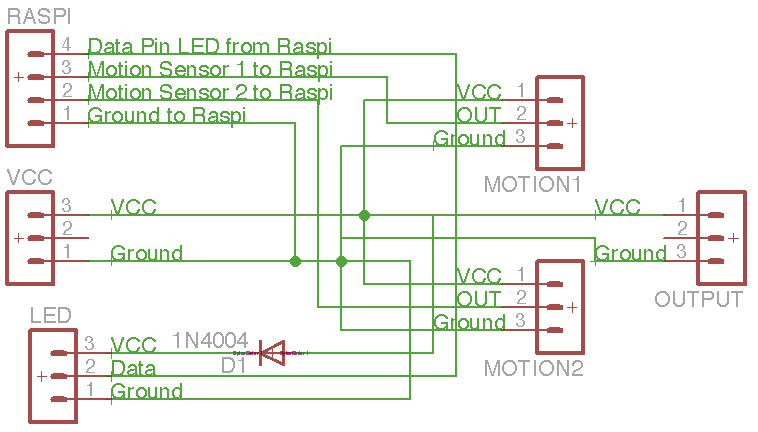
\includegraphics[width=0.9\textwidth]{./data/eagle.png}
		\caption{Schaltplan Steckplatine}
	\end{minipage}
\end{figure}

\textbf{I.II Platinenlayout}\\

\begin{figure}[h]
	\begin{minipage}{0.7\textwidth}
		\centering
		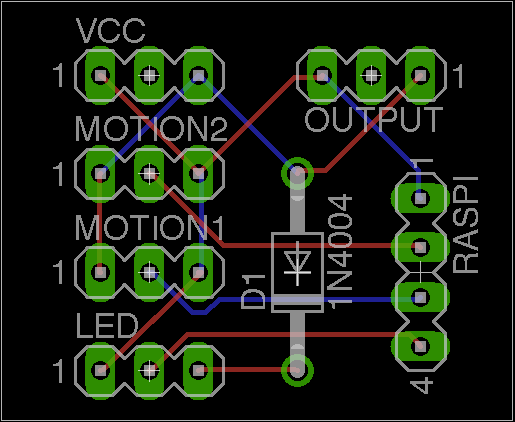
\includegraphics[width=0.7\textwidth]{./data/layout.png}
		\caption{Platinenlayout Steckplatine}
	\end{minipage}
\end{figure}

\pagebreak
\subsection*{II. Umsetzung}
\textbf{II.I Skizze des Testaufbaus}\\
\begin{figure}[h]
	\begin{minipage}{0.7\textwidth}
		\centering
		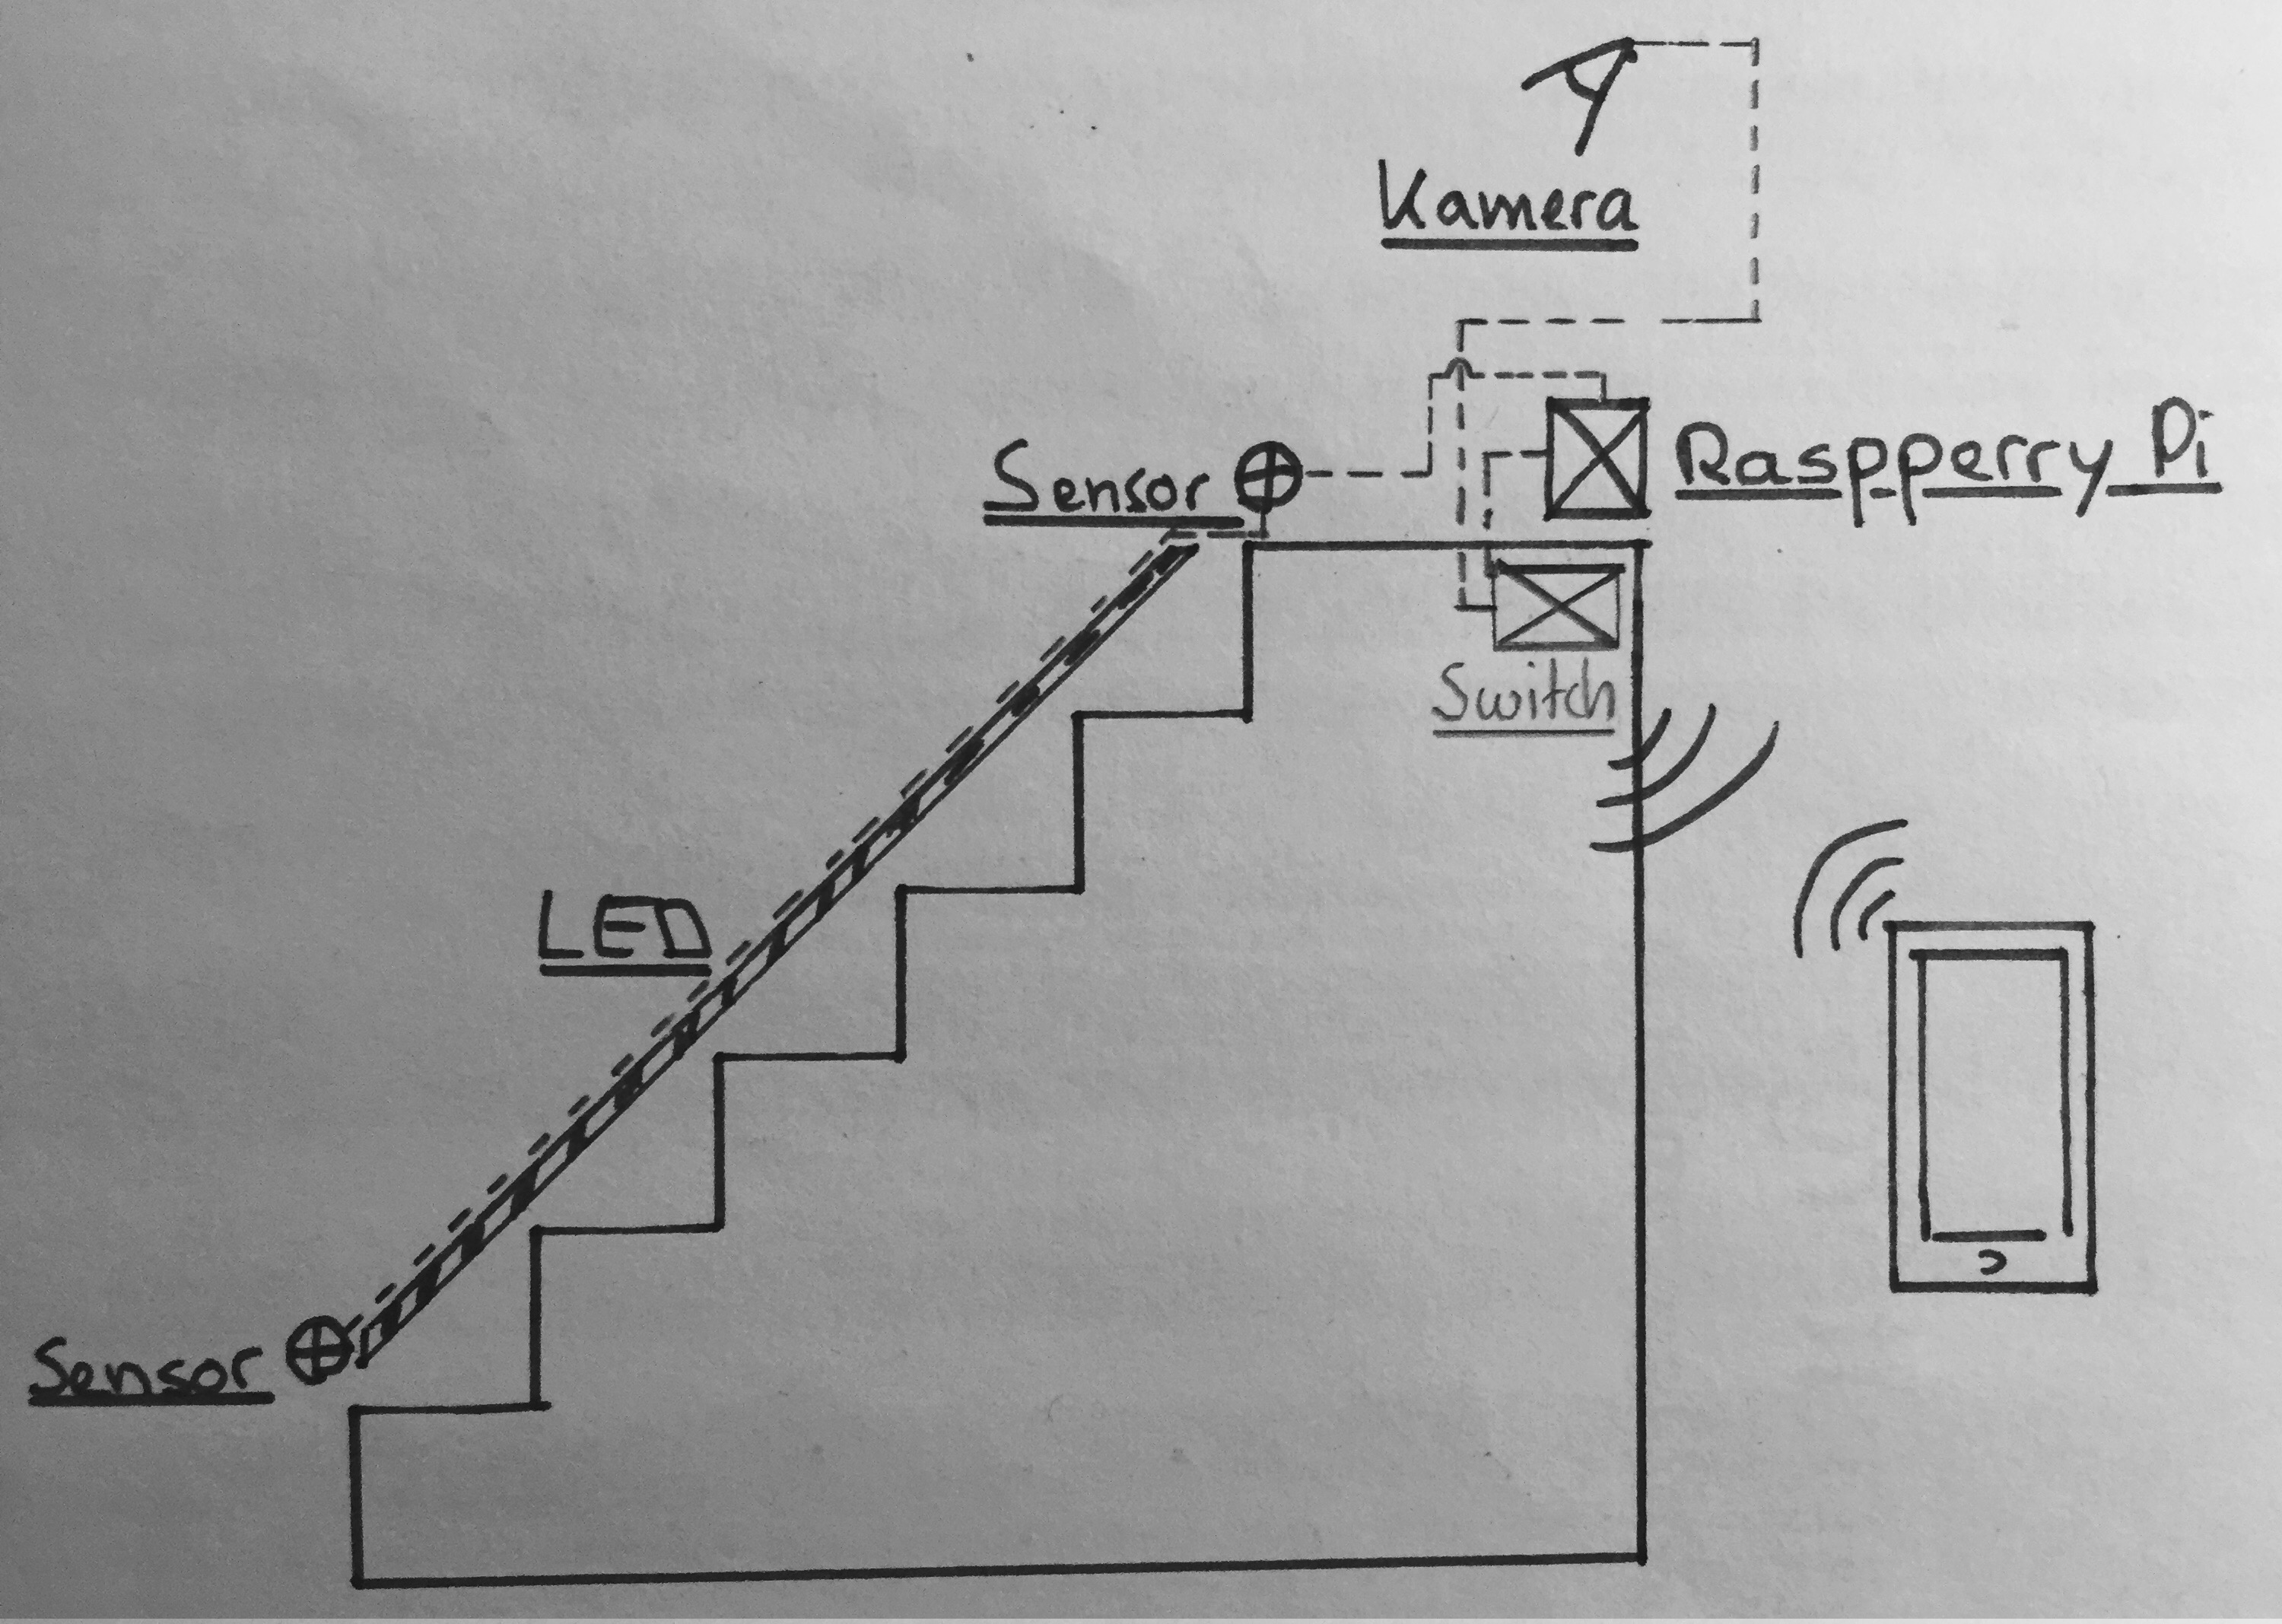
\includegraphics[width=0.7\textwidth]{./data/praxis0.jpg}
		\caption{Skizze des Aufbaus}
	\end{minipage}
\end{figure}

\textbf{II.II Kamera}\\
\begin{figure}[h]
	\begin{minipage}{0.7\textwidth}
		\centering
		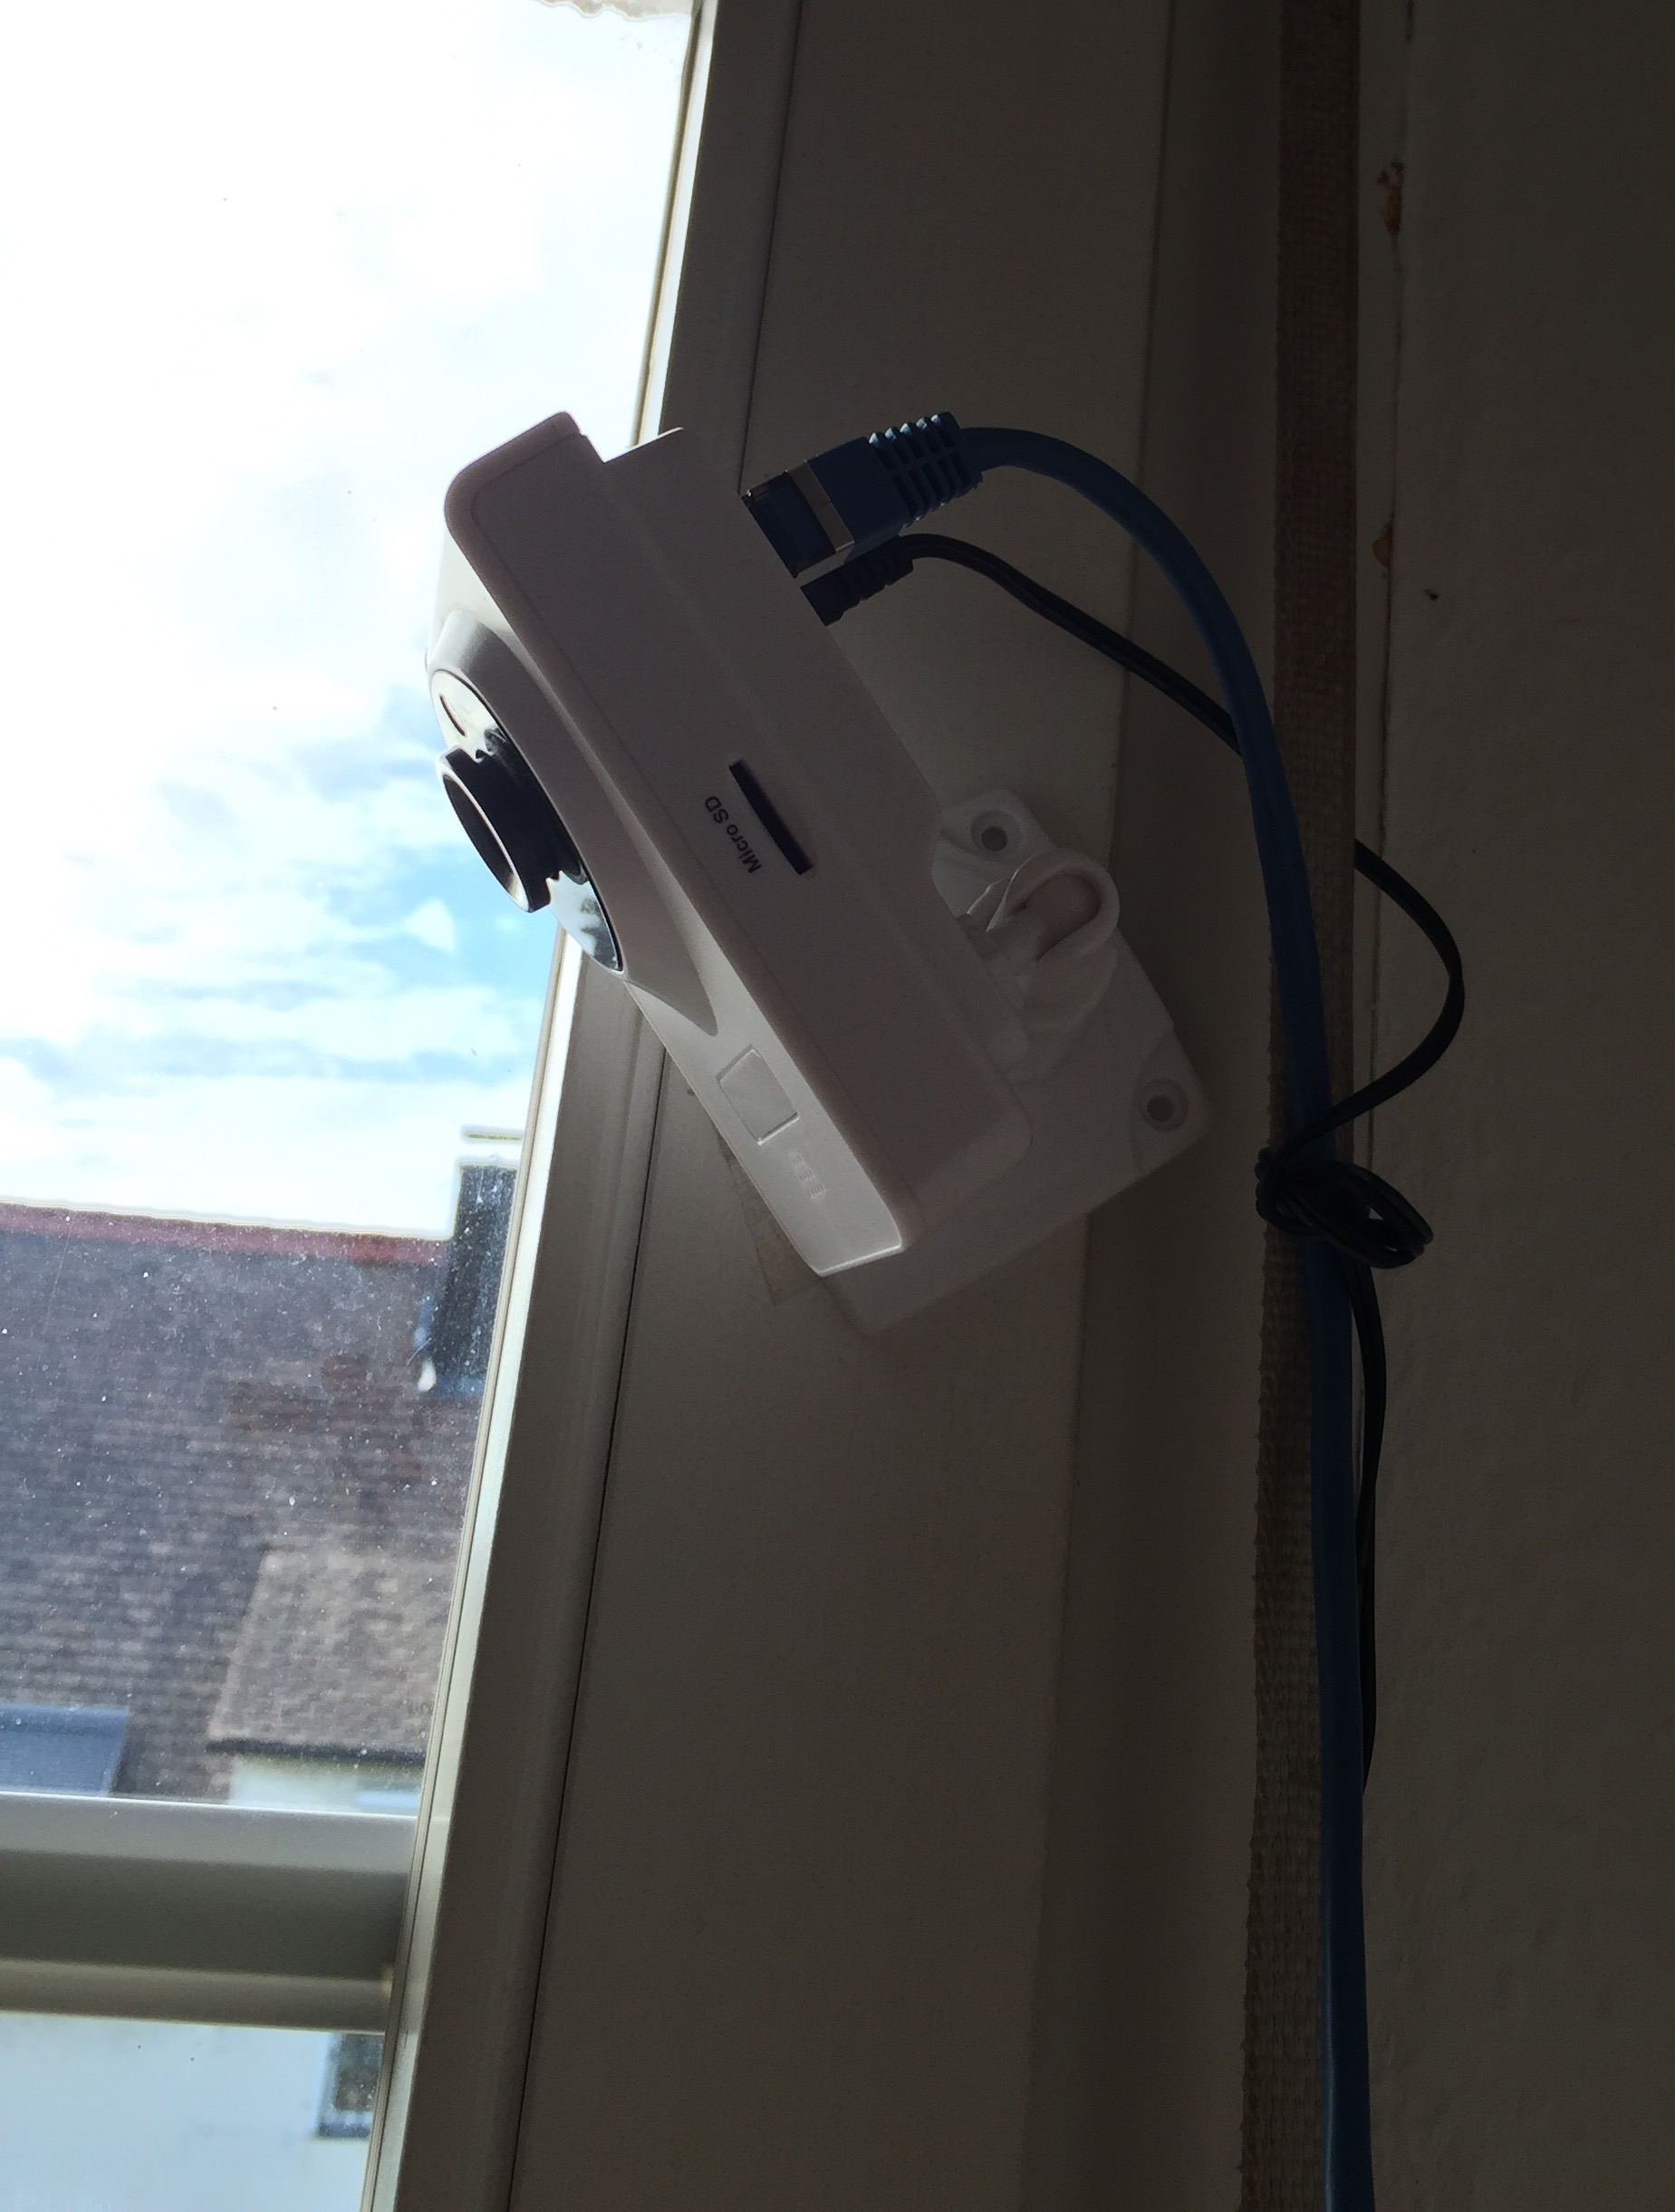
\includegraphics[width=0.7\textwidth]{./data/praxis2.jpg}
		\caption{Kamera im Testaufbau}
	\end{minipage}
\end{figure}
\clearpage
\pagebreak

\textbf{II.III Aufbau Raspberry Pi}\\
\begin{figure}[h]
	\begin{minipage}{0.7\textwidth}
		\centering
		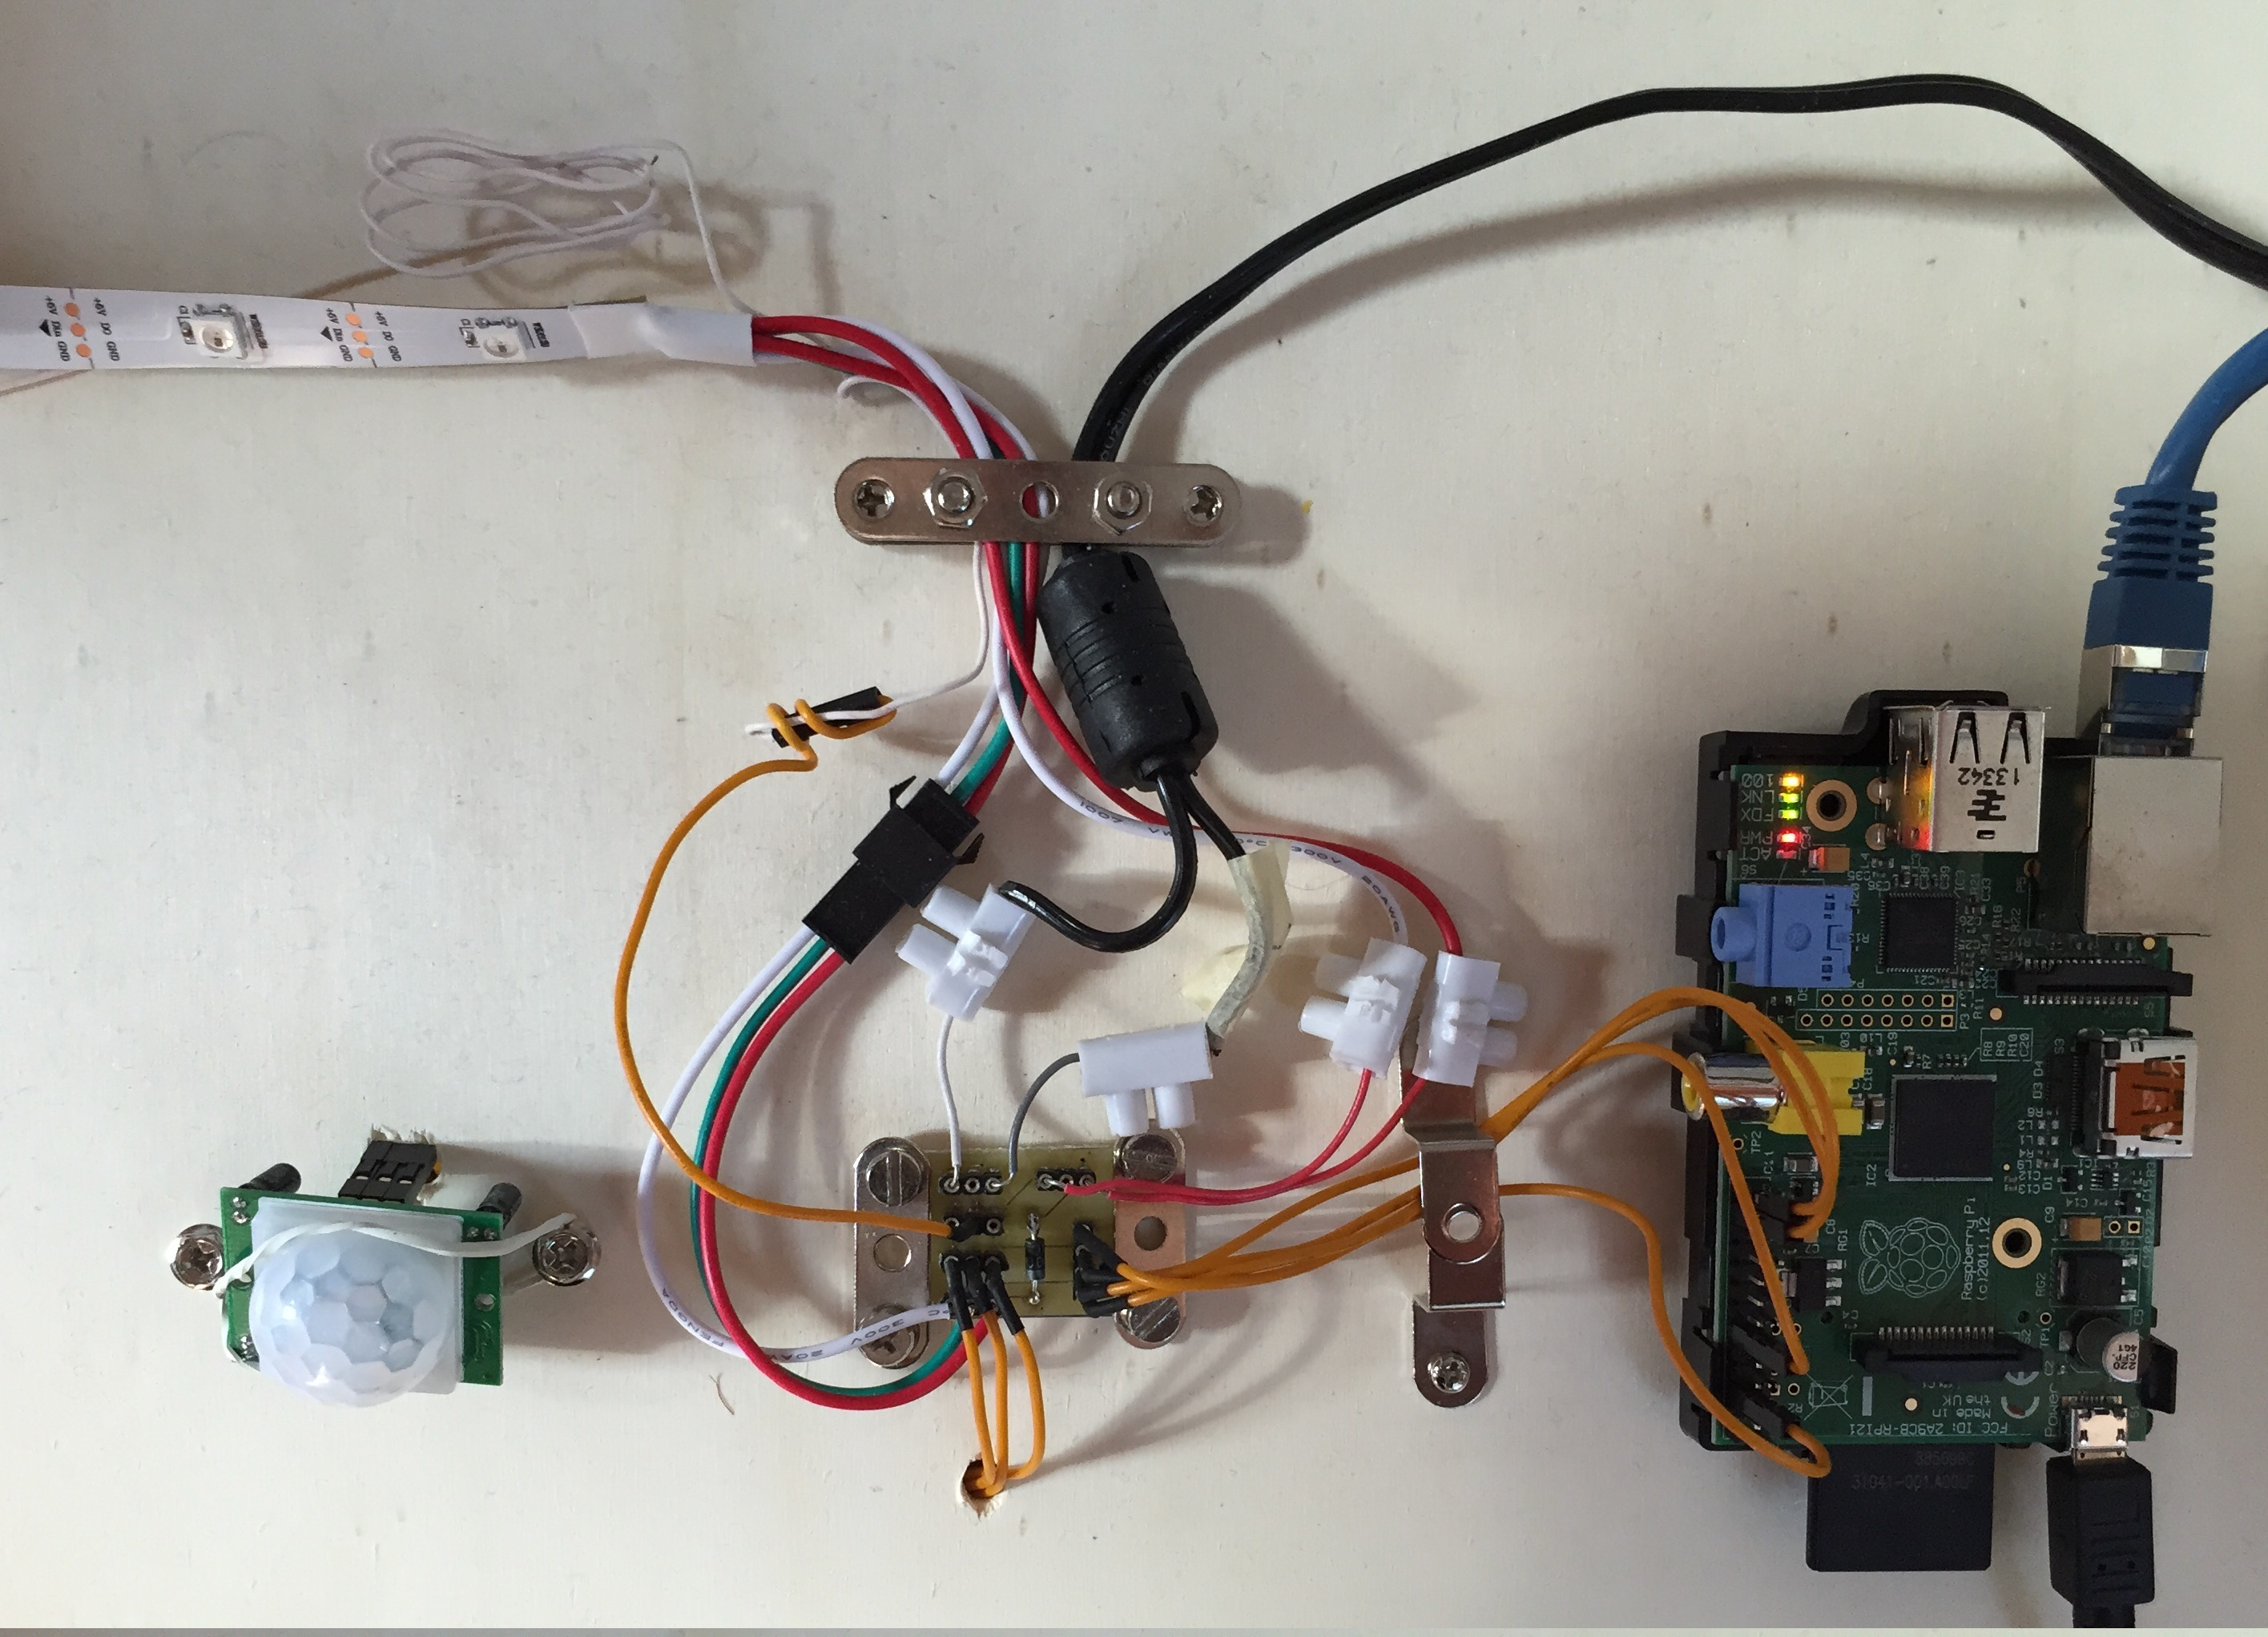
\includegraphics[width=0.7\textwidth]{./data/praxis1.jpg}
		\caption{Aufbau Raspberry Pi und Steckplatine}
	\end{minipage}
\end{figure}

\textbf{II.IV Live View}\\
\begin{figure}[h]
	\begin{minipage}{0.6\textwidth}
		\centering
		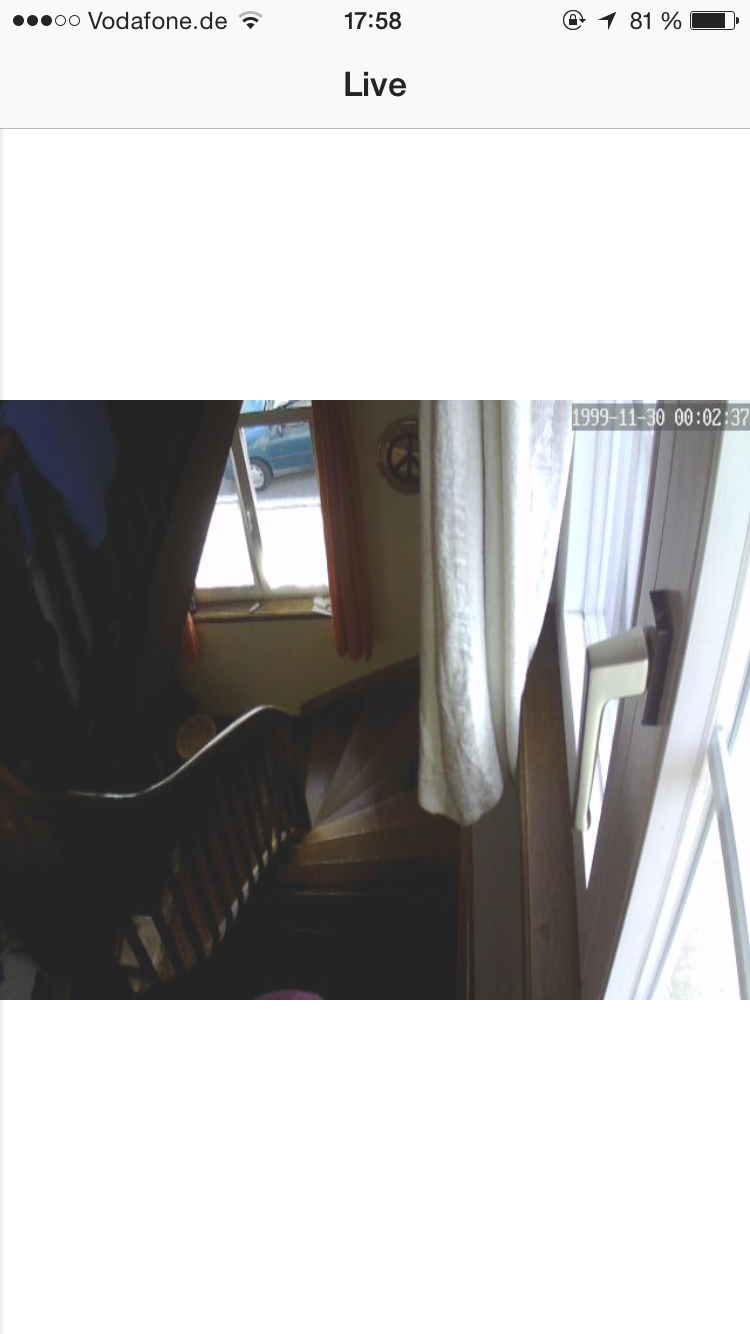
\includegraphics[width=0.6\textwidth]{./data/praxis3.jpg}
		\caption{Live-View im Testaufbau}
	\end{minipage}
\end{figure}
\clearpage
\pagebreak

\textbf{II.V Aufbau Led und Sensoren}\\
\begin{figure}[h]
	\begin{minipage}{0.9\textwidth}
		\centering
		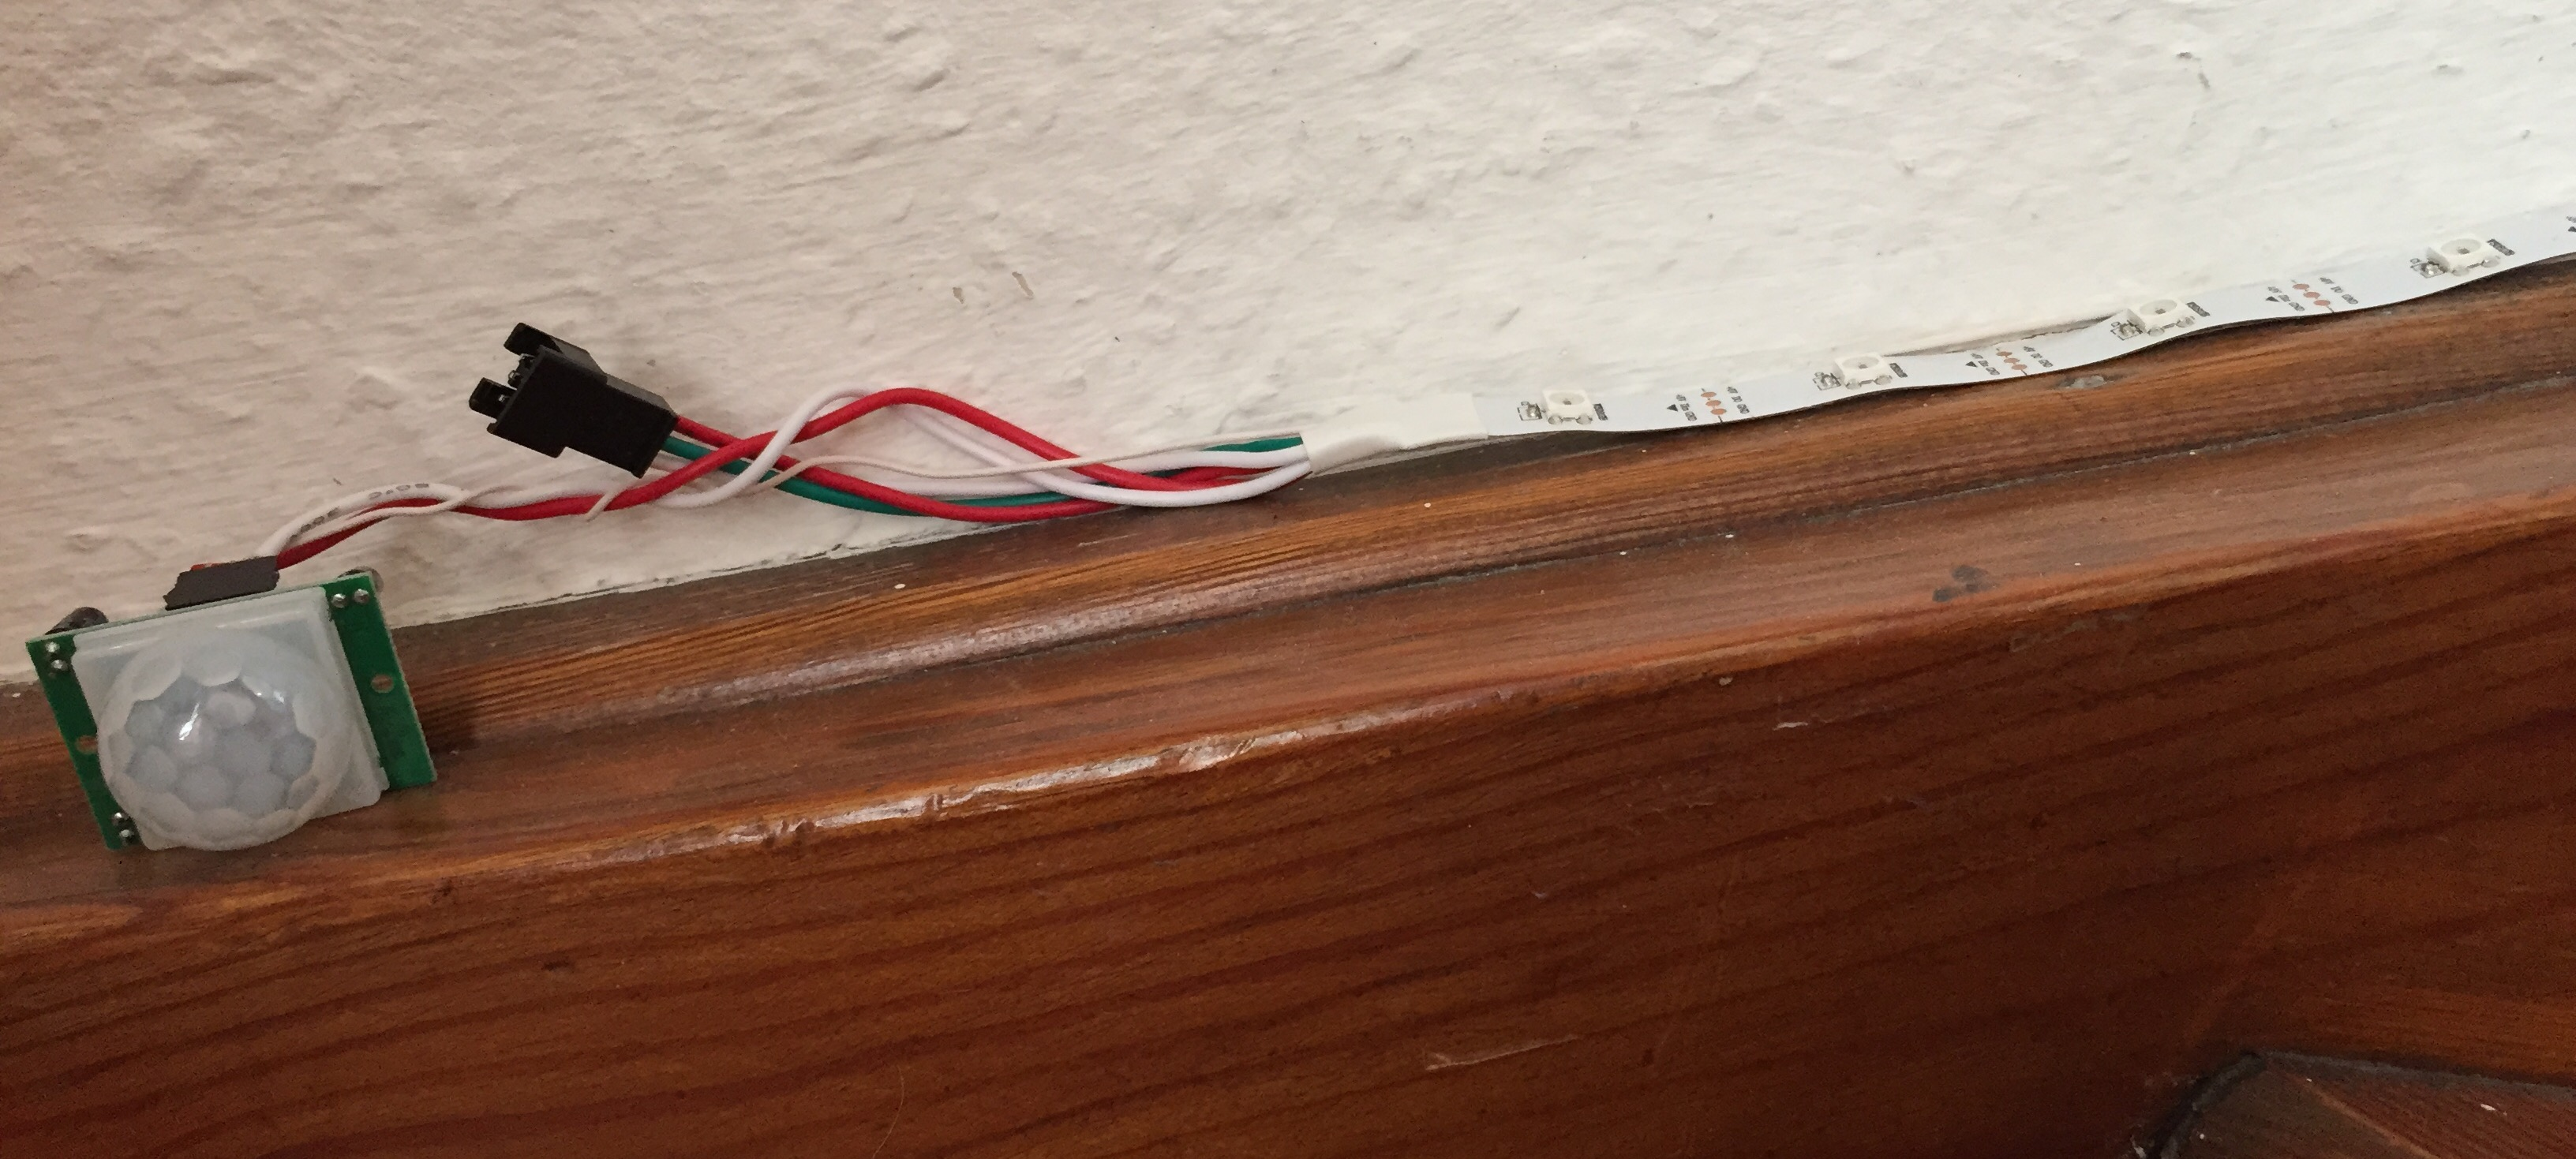
\includegraphics[width=0.9\textwidth]{./data/praxis4.jpg}
		\caption{Bewegungssensor im Testaufbau}
	\end{minipage}
\end{figure}
\begin{figure}[h]
	\begin{minipage}{0.9\textwidth}
		\centering
		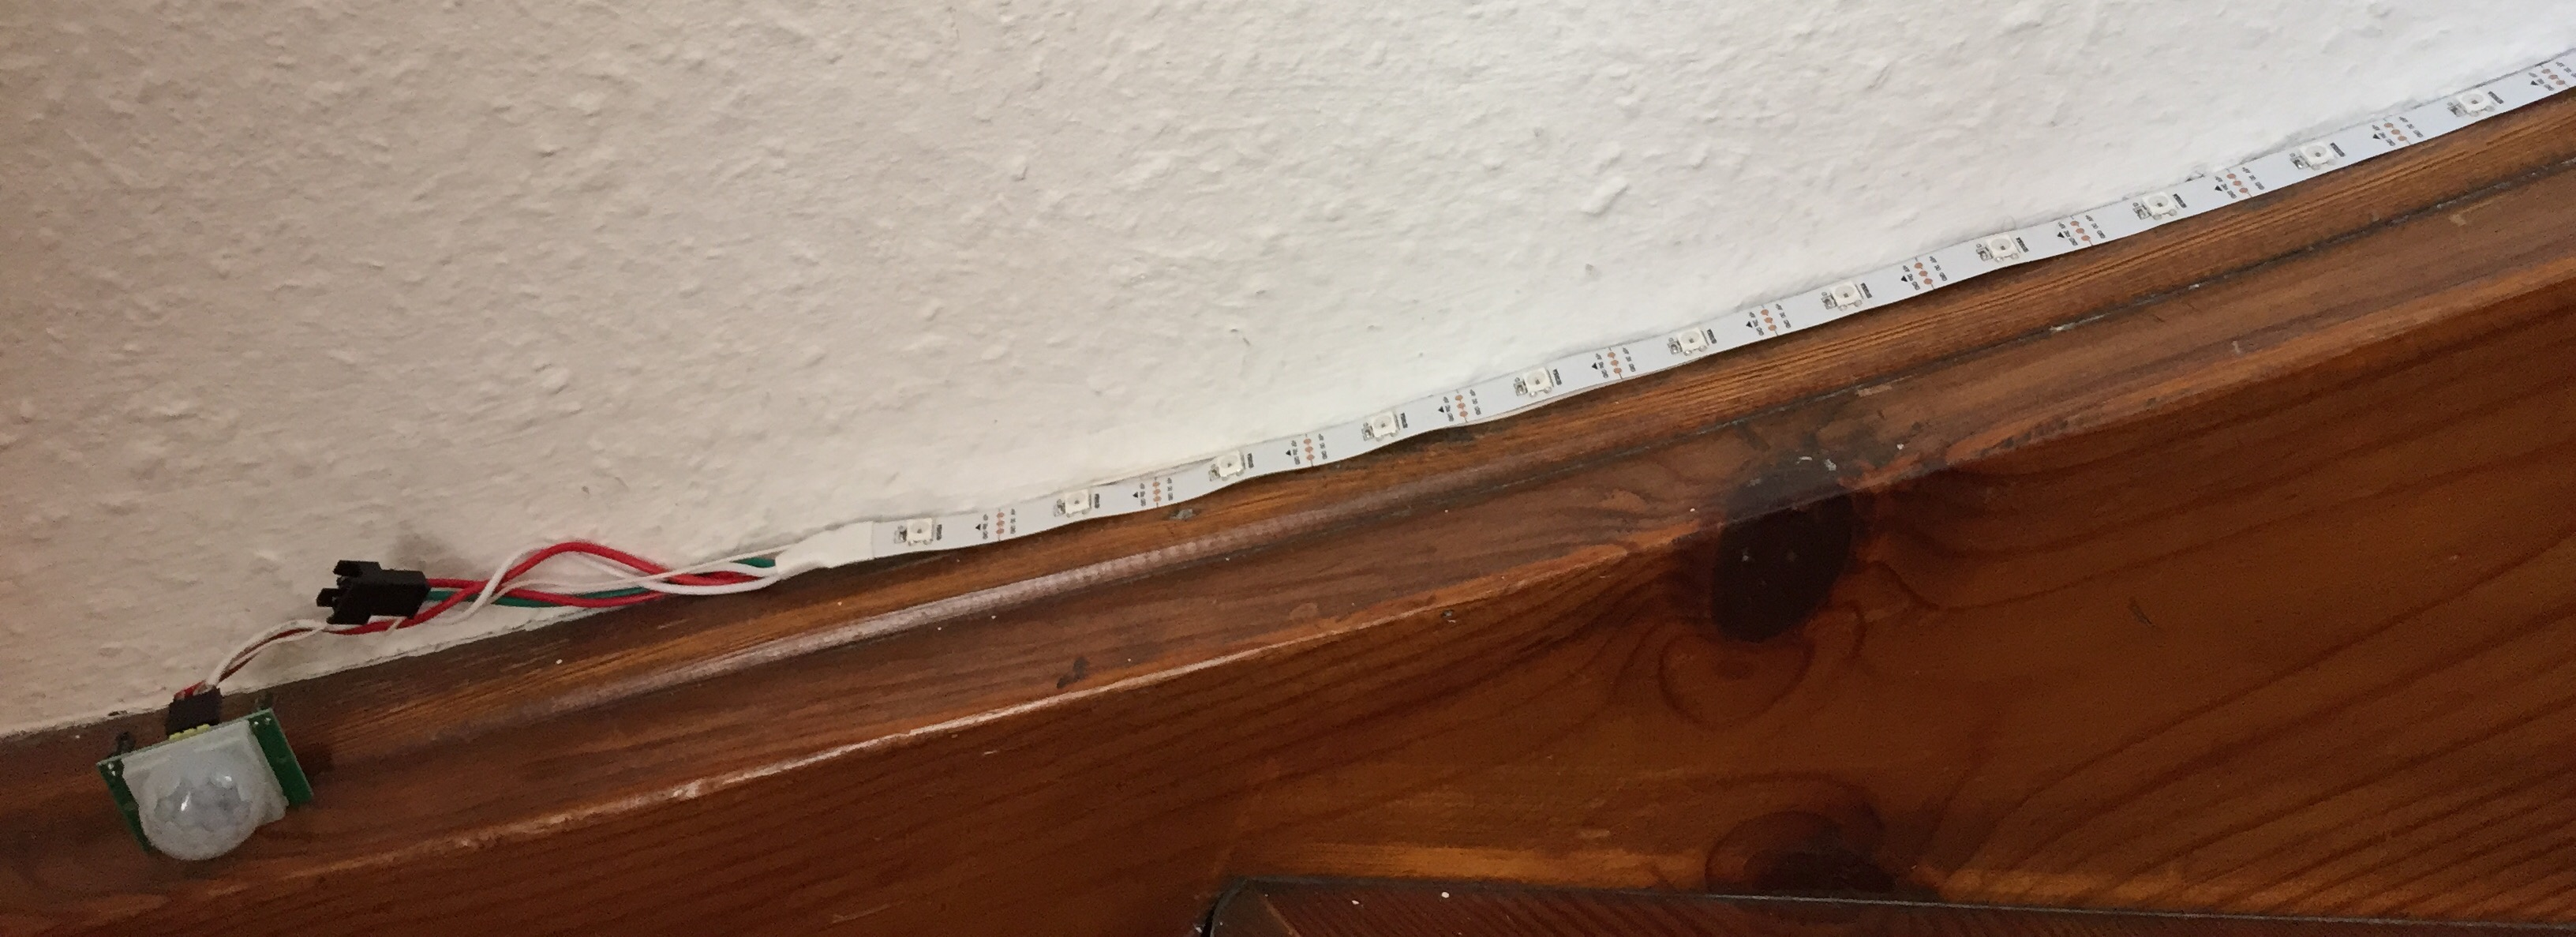
\includegraphics[width=0.9\textwidth]{./data/praxis5.jpg}
		\caption{LED-Streifen im Testaufbau}
	\end{minipage}
\end{figure}